\documentclass[11pt]{article}

\usepackage[utf8]{inputenc}
\usepackage[T1]{fontenc}

\usepackage[a4paper, left=2cm, right=2cm, top=3.5cm, bottom=3.5cm]{geometry}
\usepackage[french]{babel}

% Paragraph spacing
\setlength{\parskip}{1em}

% Fancy headers
\usepackage{fancyhdr}

% Captions for subfigures
\usepackage{subcaption}

% Footnote inside a caption
\usepackage{fnpos}
\usepackage{ftnxtra}

% Maths
\usepackage{amsmath}

% Todo notes
\usepackage{todonotes}

% Table of contents for bibliography
\usepackage[nottoc]{tocbibind}

% Inline monospace font
\def\code#1{\texttt{#1}}

% Figures
\usepackage{graphicx}

% Draw figures
\usepackage{tikz}

% Tikz node rotation
\usetikzlibrary{positioning}

% Usage: \rotnode[options]{rotation}{text}
\newcommand\rotnode[3][]{%
    \node [#1, opacity=0.0] (tmp) {#3};
    \node [draw, rotate around={#2:(tmp.center)}] at (tmp) {#3};
}

% Clickable links
\usepackage{hyperref}

% Table of contents depth
\setcounter{tocdepth}{2}

% Inline code
\usepackage{listings}
\usepackage{color}

\title{Principes et méthodes statistiques}

\author{William SCHMITT}
\date{2018-2019}

\begin{document}
\maketitle

\tableofcontents

\section{Introduction}

\subsection{Exemples}
\paragraph{Studio de musique} Mesures de bruits pour construire un studio, la
rue est au maximum à 74 dB, après 20 mesures. 74 dB est le seuil dérangeant 
les enregistrements. On peut calculer à la fin de ce cours la probabilité 
de subir des nuisances > 74 dB.

\paragraph{Sondage} Suite à un sondage (51/49), on peut estimer le risque à 
prendre pour pouvoir affirmer que le candidat annoncé gagnant sera effectivement
élu.

\subsection{Rappel des concepts abordés l'an dernier}
\begin{figure}
    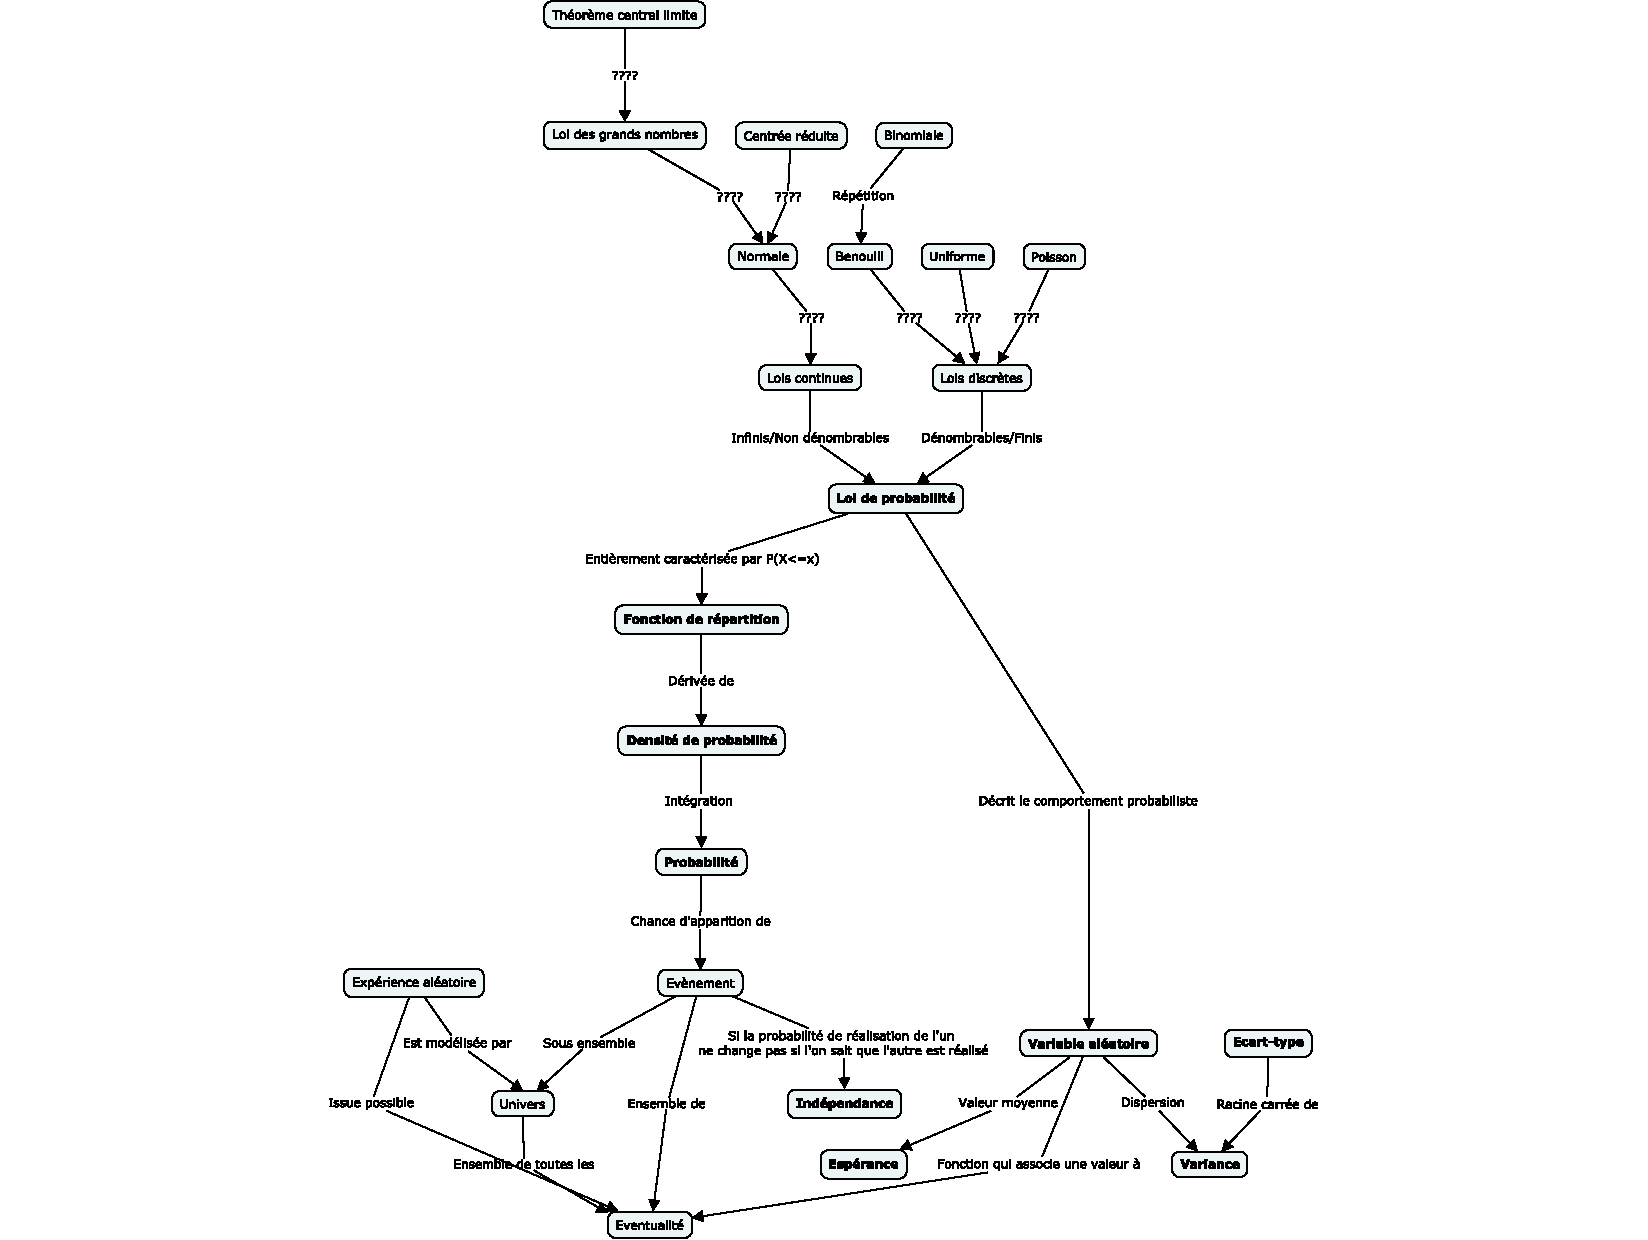
\includegraphics[scale=.65]{img/mindmap-1AA-probas.pdf}    
\end{figure}


\begin{itemize}
    \item Lois de probabilité
    \begin{itemize}
        \item continues
        \begin{itemize}
            \item Normale
            \item Poisson
        \end{itemize}
        \item discrètes
        \begin{itemize}
            \item Bernoulli
            \item Binomiale
            \item Géométrique
        \end{itemize}
    \end{itemize}
    \item Indicateurs 
    \begin{itemize}
        \item espérance
        \item variance
        \item écart-type
    \end{itemize}
    \item Fonctions génératrices (des moments)
    \item Fonction de répartition
    \item Fonction de densité
    \item Loi des grands nombres
    \item Théorème central limite
    \item Indépendance de variables aléatoires
\end{itemize}

\subsection{Les deux dés}
Expérience aléatoire : on lance deux dés, un rouge et un bleu, à six faces et
équilibrés.
On introduit les variables aléatoires suivantes :
\begin{itemize}
    \item B : valeur du dé bleu
    \item R : valeur du dé rouge
    \item S : somme des deux valeurs
\end{itemize}

\subsubsection{Question} Les variables aléatoires B et R sont égales ? 
\begin{itemize}
    \item Vrai
    \item Faux
    \item Autre
\end{itemize}

\subsubsection{Retours}
La variable aléatoire \textbf{est une fonction}, qui à chaque probabilité fait
correspondre une valeur.
\begin{align*}
    B: &\Omega \to \{1,2,3,4,5,6\} \\
    &\omega \mapsto B(\omega) \\
    &(b, r) \mapsto b
\end{align*}

\todo[inline]{Il manque un bout ici.}

\begin{align*}
    \omega = (b, r) \\
    S \mapsto b+r
\end{align*}

avec b: valeur du dé bleu, r: valeur du dé rouge.

Elles ne sont pas égales : sinon les valeurs prises seraient toujours égales.
C'est-à-dire que si elles étaient égales, si le dé rouge tombait sur 1, le dé
bleu tomberait également sur 1.

Elles ont néanmoins la même loi.

\subsubsection{Indépendance} Soient deux évènements, sont-ils indépendants ?

\paragraph{Exemple 1}
\begin{itemize}
    \item $A = \{\text{Somme} = 3\}$
    \item $B = \{\text{Dé rouge} = 4\}$
\end{itemize}
Les évènements ne sont pas indépendants, trivialement.


\paragraph{Exemple 2}
\begin{itemize}
    \item $C = \{\text{Somme est paire} \}$
    \item $D = \{\text{Dé rouge pair} \}$
\end{itemize}
C, comme D, sont de probabilité $\frac{1}{2}$. La réponse est complexe car D a
une influence sur C. Néanmoins, les probabilités ne sont pas affectées : les
évènements C et D sont donc bel et bien \textbf{indépendants}.

\end{document}